\documentclass[dvipdfmx]{jarticle}
\usepackage{graphicx}
\usepackage[top=30truemm,bottom=30truemm,left=25truemm,right=25truemm]{geometry}
\usepackage{listings,jvlisting}
\usepackage{url}

\lstset{
  basicstyle={\ttfamily},
  identifierstyle={\small},
  commentstyle={\smallitshape},
  keywordstyle={\small\bfseries},
  ndkeywordstyle={\small},
  stringstyle={\small\ttfamily},
  frame={tb},
  breaklines=true,
  columns=[l]{fullflexible},
  numbers=left,
  xrightmargin=0zw,
  xleftmargin=3zw,
  numberstyle={\scriptsize},
  stepnumber=1,
  numbersep=1zw,
  lineskip=-0.5ex
}

\makeatletter
\newcommand{\subsubsubsection}{\@startsection{paragraph}{4}{\z@}%
  {1.0\Cvs \@plus.5\Cdp \@minus.2\Cdp}%
  {.1\Cvs \@plus.3\Cdp}%
  {\reset@font\sffamily\normalsize}
}
\makeatother
\setcounter{secnumdepth}{4}

\begin{document}
\begin{titlepage}
    \begin{center}
        {\huge 情報科学演習D 課題3レポ―ト}
        \vspace{180pt}\\
        \begin{tabular}{rl}
            氏名 & 山久保孝亮\\
            所属 & 大阪大学基礎工学部情報科学科ソフトウェア科学コース\\
            メールアドレス & u327468b@ecs.osaka-u.ac.jp\\
            学籍番号 & 09B22084\\
            提出日 & \today\\
            担当教員 & 桝井晃基 松本真佑
        \end{tabular}
    \end{center}
\end{titlepage}
\section{システムの仕様}
課題3の外部仕様は以下のようになる.
\begin{itemize}
  \item 第一引数で指定されたtsファイルを読み込んでい未解析を行い,意味的に正しい場合は文字列"OK"を,正しくない場合は文字列"Semantic Error"に続いて対応する行番号を返す.
  \item 複数の意味的誤りが含まれる場合では,最初に見つけた誤りのみを出力する.
  \item 意味解析よりも先に構文解析を適用し,構文エラーを見つけると”Syntaxerror: line”という文字列に続いて対応する行番号を返す.
  \item 入力ファイルが見つからない場合は文字列”File not Found”を返す.
\end{itemize}
\section{課題達成の方針と設計}
課題3のテストケースをパスするために実装した機能は以下の通りである.
\begin{enumerate}
  \item 変数が重複して定義されない.
  \item 未定義の変数及び関数を参照しない.
  \item 型における制約を守る.
  \item 代入文の左辺に配列型の変数名を使用しない.
\end{enumerate}
課題3では課題2のparser.javaのプログラムの一部を変更して実装した.上記の機能を満足するために変
更及び追加した方針は以下の通りである.
\begin{itemize}
  \item 変数,関数を記憶するための表を作成する.今回作成した表は言語処理工学Aの授業スライドを参考にして作成した.
  この表により変数の二重定義,未定義の変数及び手続きの参照を防止できる.それぞれの表の構成要素は以下の表の通りである.
  \begin{table}[h]
    \centering
    \begin{tabular}{|c||c|c|c|}
      \hline
      変数表 & 変数名 & 変数の型 & 変数のサイズ\\\hline
      関数表 & 関数名 & 引数の型 & null\\\hline
    \end{tabular}
    \caption{それぞれの表の構成要素}
  \end{table}
  \\null は要素が存在しないことを,つまり関数表には二つの要素しか存在しないことを表す.
  変数のサイズには配列の際は要素数を,配列でなければ1を格納する.
  \item 変数の宣言において,指導書よりプログラムの宣言と手続きの宣言で処理を分ける必要がある.
  したがって,変数表はグローバル変数用のものとローカル変数用のものをそれぞれ用意した.これにより,グローバル変数を宣言する処理の際はglobal\_variable\_tableを,ローカル変数を宣言する処理の際はlocal\_variable\_tableを参照することによって要件を満足することができた.
  \item 式,単純式,項,因子,定数を判定するメソッドが型を返すようにした.課題2では構文定義を判定するメソッドはすべてvoid型であったが,前述のメソッドが”integer”,”char”,”boolean”のいずれかをString型で返すようにした.
  これにより,各被演算子の型を把握することができるので,型の整合性がとれているのか,特定の演算子に適した型が使用されているのかを判定する.
\end{itemize}
\section{実装プログラム}
今回実装したプログラムは以下の通りである.
\subsection{表の作成}
2で記述したように,変数の情報を記録しておくために表を作成した.それぞれの表に対応するvariable,functionというクラスを作成し,それぞれグローバル変数のリストとしてどのメソッドからでも参照できるようにした.
それぞれのクラス内の変数は表1に対応しており,それぞれのクラス内で以下のようなメソッドを作成した.
\begin{lstlisting}
  public Type get_A_B(){
    return B;
  }
\end{lstlisting}
ここではAがどの表であるか,Bが表のどの変数であるかに対応している.これにより,例えばvariableというリストのi番目の要素に対して上記のメソッドを実行すればi番目のBの値を参照できるようになる.
\subsection{表への格納}
変数表,関数表への格納は以下の図1のフローチャートに従って実行される.
\begin{figure}[h]
  \centering
  \begin{minipage}[b]{0.49\columnwidth}
      \centering
      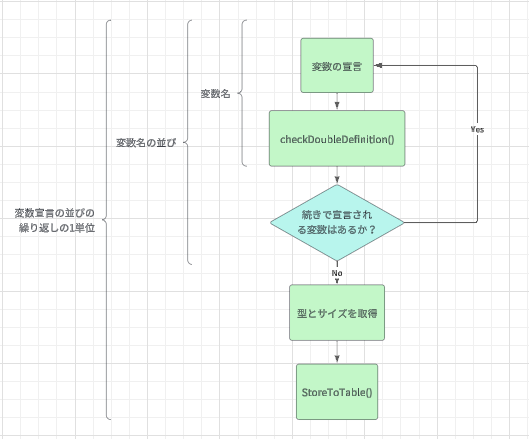
\includegraphics[width=0.9\columnwidth]{hurotya.png}
      \caption{変数宣言の並びの繰り返しの1単位}
      \label{fig:a}
  \end{minipage}
  \begin{minipage}[b]{0.49\columnwidth}
      \centering
      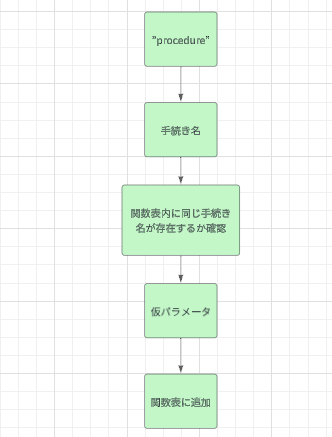
\includegraphics[width=0.6\columnwidth]{hurotya1.png}
      \caption{副プログラム頭部}
      \label{fig:b}
  \end{minipage}
  \end{figure}
  \\図1は1回以上繰り返される変数宣言の並びの繰り返しの1単位の処理を表している.checkDoubleDefinition()とStoreToTable()はそれぞれ二重定義の処理と変数表への格納の処理を行う.
また,ここではグローバル変数としてlist\_of\_variablenameというString型のリストを使用し,checkDoubleDefinition()の結果二重定義でなければadd()を使用し追加している.
ここでいきなり変数表に格納しない理由は,この段階では変数名がわかっただけでありその変数の型やサイズが不明であるためである.したがって,型とサイズが判明してからStoreToTable()を呼び出している.
以下ではcheckDoubleDefinition()とStoreToTable()の詳細について述べる.
\begin{itemize}
  \item checkDoubleDefinition()では変数名が二重定義されていないかを確認している.引数には宣言された変数名が渡されており,それが各表の名前と一致していないかを確認する.
  一致している場合即ち二重定義されている場合,文字列"NO"を返し,一致していない場合文字列"YES"を返す.
  まず関数名,list\_of\_variable\_nameと一致していないかを確認する.繰り返し文と3.1で紹介したメソッドを用いて表に格納された関数名を取り出して比較する.
  そして,プログラムの宣言の際はグローバル変数用の表と,手続きの宣言の際はローカル変数用の表と一致していないかを確認する.
  \item StoreToTable()では表への格納を行っている.引数のlistは二つの要素があり,一つ目は格納する変数の型,二つ目は格納する変数のサイズである.
  global\_flagによってグローバル変数用の表に格納するか,ローカル変数用の表に格納するかを分岐させている.このフラグはプログラムの宣言の際に立ち上げ,手続きの宣言の際には下げられている.また,list\_of\_variablenameはこのメソッドが呼び出されるたびに初期化される.
  これは,新たな変数宣言の繰り返し単位が存在した場合に再度表に追加されてしまうことを防ぐためである.
\end{itemize}
関数表への格納は図2のように副プログラム頭部のメソッドに処理を追加して実装した.
関数名を関数表へ追加する前に同じ手続き名が存在しないかを確認する.確認は変数の際と同様にループを用いて実装した.仮パラメータの処理については変数の表への追加と基本的に同じだが,
型をリストにして格納している.つまり一つの関数名に対して一つの仮パラメータのリストが存在するということである.
これは考察で述べる仮パラメータと実引数との整合性を保つために実装している.
\subsection{未定義の変数の参照}
未定義の変数の参照を防ぐためにcheckVariable()というメソッドを定義した.これは変数の定義の後に呼び出される.引数として識別子が渡され,
その文字列が変数表内で定義済みかどうかを判定する.定義されていない場合は文字列"NO"を,定義されている場合はその変数の標準型を文字列として返す.
ここでは変数のサイズが1かどうかも判定され,1でなければグローバル変数であるarray\_flagが1となる.これを用いた具体的な処理は後述する.
\subsection{型の制約}
ここでは,各演算子において被演算子の型と結果の型の整合性を確認する処理方法について記述する.
\begin{itemize}
  \item まず,被演算子の型の整合性について記述する.加法演算子と乗法演算子の場合"and"と"or"の場合はboolean型を,それ以外の場合はinteger型を,被演算子の型として処理するようにした.
  また,被演算子同士の型が一致している必要があるので,最初の被演算子の型を格納する変数first\_typeと,もう一つの被演算子の型を格納する変数second\_typeが一致しているかどうかを判定する.
  式や単純式,項のように,0回以上の繰り返しがある場合はfirst\_typeは変えずに,新たな被演算子が現れるたびにsecond\_typeを更新し一致しているかを判定することで全ての被演算子の型が一致していることを確かめた.
  
  \item 次に,結果の型の整合性について記述する.加法演算子と乗法演算子の場合"and"と"or"の場合はboolean型を,それ以外の場合はinteger型を結果の型として処理するようにした.また,
  関係演算子の結果はboolean型として処理するようにした.
\end{itemize}
\subsection{左辺の型の分類}
代入文の構文定義において,左辺が純変数か添え字付き変数かを判定する処理が行われる.このとき,純変数として本来は配列型の変数名が使用されないようにするために3.2で記述したarray\_flagを使用する.
構文的に純変数であると判明した後にこのarray\_flagがtrueとなっているかを判定する.これにより,上記のテストケースに対応することができるようになる.なお,array\_flagはcheckVariable()が呼ばれるたびにfalseに初期化されるため,
各変数の参照に対して更新される.
\section{考察}
今回のテストケースは最低限満たす必要のあるものであったが,実際にはほかにも意味エラーが発生することが考えられる.以下は私が追加で考えられる意味エラーのパターンである.
\begin{itemize}
  \item 配列の定義の際に,添え字の最小値と最大値の大小関係が逆転している.
  \item 仮パラメータと実パラメータの整合性がとれていない.
\end{itemize}
具体的な実装方法は以下のとおりである.
\begin{itemize}
  \item 添え字の最小値と最大値をそれぞれ保持しておき,大小比較をして最大値>最小値でなければ意味エラーとすることで実装した.
  \item 3.2で記述したように関数表における引数の型をリストとして定義し保持しておく.手続き呼び出し文において式の並びを実装したメソッドの返り値を型のリストに変更し,
  返された型のリストと,関数表に保持しているリストの要素が同じであるかをループを使って確認することで実装した.
\end{itemize}
以上のパターンの意味エラーの処理を作成して,今後の拡張内容として以下のような点が挙げられると考えた.
\begin{enumerate}
  \item 意味エラーの出力だけでなく,どのようなエラーなのか(未定義の変数を参照しているのか,二重定義をしているのか等)を出力する.これにより,プログラマにどのような意味エラーが起きているのかを伝えられるためより親切な設計にすることができる.また,出力する文字列を変更するだけでよいので
  実装の難易度は低いと考えられる.
  \item 変数表に格納されている識別子名の内,参照されていない変数は取り除くもしくは表から削除する.具体的には参照されたかどうかを表すフラグを表に追加し,参照された場合はそのフラグを1にそれ以外は0にすることで,
  checkerを実行した後にフラグが0になっている変数は使用されていないということになるので消去しても問題がないと考えらえる.
\end{enumerate}
\section{感想}
課題3を通して学んだ感想としては,テストファーストな開発がとても効率的であったということである.課題2においてウォータフォール型の開発をしたことの反省から
テストファーストな開発を試してみて,かなり効率的に実装を進めることができたと感じた.課題4でも同様にテストファーストな開発で進めていきたいと思う.
\begin{thebibliography}{1}
    \bibitem{1} 言語処理工学A 講義スライド
    \bibitem{2} 情報科学演習D 指導書
\end{thebibliography}
\end{document}